\documentclass[a4paper,twoside]{article}

\usepackage{epsfig}
\usepackage{subfigure}
\usepackage{calc}
\usepackage{amssymb}
\usepackage{amstext}
\usepackage{amsmath}
\usepackage{amsthm}
\usepackage{multicol}
\usepackage{pslatex}
\usepackage{apalike}
\usepackage{SciTePress}
\usepackage[small]{caption}
\usepackage{epstopdf}
\usepackage[utf8]{inputenc}
\usepackage[ngerman]{babel}
\usepackage{url}
\usepackage{hyperref}
\usepackage{listings}
\usepackage{enumerate}
\usepackage{multicol}
\usepackage{tabularx}
\usepackage{array}

\lstdefinestyle{myCustomUseStyle}{
  stepnumber=1,
  numbersep=10pt,
  basicstyle=\footnotesize\ttfamily,
  tabsize=3,
  showspaces=false,
  showstringspaces=false,
  breaklines=true
}

\subfigtopskip=0pt
\subfigcapskip=0pt
\subfigbottomskip=0pt

\pagestyle{plain}

\begin{document}

\title{\uppercase{Modellgetriebene Entwicklung einer mobilen Applikation mit JUSE4Android}}

\author{\authorname{Jano Espenhahn, Tobias Franz and Franziska Krebs}
\affiliation{Fachhochschule Brandenburg, Fachbereich Informatik und Medien}
\email{\{espenhah, franzt, krebsf\}@fh-brandenburg.de}
}

\keywords{MDA, UML, USE, OCL, Android}

\abstract{ein deutsches Abstract: Entwicklung einer Applikation, USE-Spezifikation zur Definition eines Klassendiagramms; OCL-Constraints oben drauf;Im Anschluss Generierung der Anwendung mit Hilfe von JUSE4Android. Untersuchung der Anwendung anhand bestimmter Fragestellungen   }{ein englisches Abstract}


\onecolumn \maketitle \normalsize \vfill
\pagestyle{plain}
\section{\uppercase{Einleitung}}
\label{sec:introduction}
\noindent Zitat Test
\cite{SilvaMasterThesis}

\section{\uppercase{Beschreibung der Anwendung}}
\noindent
Das Beispiel wurde aus dem Artikel \cite{Gui06} entnommen. Es handelt sich um ein fiktives Programm der Regierung zur Kontrolle der Eispartikel in der Luft. Wenn die Konzentration zu niedrig ist, bedeutet das, dass die Bevölkerung zu wenig Eiscreme isst, was eine Menge an Risiken für die Umwelt und die öffentliche Ordnung darstellt. Um die Eispartikel in der Luft zu überwachen, hat der Staat Kontrollstationen im gesamten Land verteilt aufgestellt. Für jede Station gibt es einen festgelegten Zielwert der Eispartikel. Der aktuelle Wert weicht in der Regel vom Zielwert ab. 
\\
Die Anwendung ermöglicht es, neue Stationen mit Zielwerten aufzunehmen und alte Stationen zu löschen. Außerdem gibt es die Möglichkeit, eine Adresse zu einer Station anzugeben. Eine Adresse ist im Nachhinein auch wieder entfernbar. Die Erfassung von beliebig vielen Einträgen zu einer Station ist ebenfalls möglich. Auch Einträge lassen sich im Nachhinein wieder entfernen. Zudem wird für jeden Eintrag nach Eingabe des aktuellen Wertes die Abweichung zum Zielwert (im Folgenden als Varianz bezeichnet) angezeigt.


\section{\uppercase{Vorstellung USE}}
\noindent
UML based Specifiation Environment (USE) wird zur Spezifikation von Informationssystemen verwendet und wurde an der Universität Bremen entwickelt. Neben dem Einsatz für Fallstudien wird USE vor allem in der Lehre an Hochschule wie z. B. MIT, Cambridge, University of Edinburgh und University of Lisbon eingesetzt. USE basiert auf einer Teilmenge der Unified Modeling Language (UML) und der Object Constraint Language (OCL). Eine USE-Spezifikation besteht aus einer textuellen Beschreibung eines Modells, bei der Eigenschaften aus UML-Diagrammen verwendet werden. Weitere Integritätsausdrücke für ein Modell können durch die OCL definiert werden. \cite{Use07}
%Die OCL wird im späteren Kapitel (TODO) vorgestellt. 
\\

Die Abbildung~\ref{fig:Grafik1} veranschaulicht den Workflow für eine USE-Spezifikation. Ein Entwickler spezifiziert ein plattformunabhängiges (PIM) USE-Modell, welches ein System beschreibt und nutzt dafür UML- und OCL-Ausdrücke. Mithilfe von USE ist es ihm möglich, die bestimmten Anforderungen an sein System auf Erfüllung mit dem Modell zu validieren.

\begin{figure}[!h]
	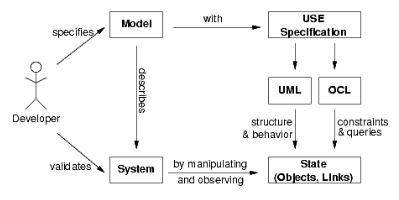
\includegraphics[scale=.7]{pics/USE_workflow.jpg}
	\caption{Workflow einer USE-Spezifikation \cite{Data07}}
	\label{fig:Grafik1}
\end{figure}

\subsection{Spezifikation} 
\label{ssec:specification}

Die textuelle Beschreibung eines Modells mit USE beginnt immer mit der Definition eines Modell-Namens. In diesem Fall ist das \textit{IceCream}. Im Anschluss folgen Klassendefinitionen mit ihren jeweiligen Attributen und Methoden. Im Beispiel hat die Klasse \textit{Station} das Attribut \textit{name} und die Operation \textit{entries} ohne Übergabeparameter. Die nachfolgenden Code-Ausschnitte verwenden lediglich UML.

\lstset{basicstyle=\tiny,style=myCustomUseStyle}
\begin{lstlisting}[caption={USE-Spezifikation der Klasse Station im Modell IceCream},label=lst:use1]
model IceCream

class Station
	attributes
		name			: String
		target		: Integer
		numberOfEntries : Integer
		meanActualValue : Real 
		meanVarianceValue :Real
	operations
		entries()	: Set(Entry) 
		calculateMeanActualValue() : Real
		calculateMeanVarianceValue() : Real
		
end
\end{lstlisting}

Klassen können untereinander in Abhängigkeit stehen. Für diese Abhängigkeiten sind Assoziationen vorgesehen. Um eine Assoziation auszudrücken, wird zuerst eine weitere Klasse \textit{Address} eingeführt.

\begin{lstlisting}[caption={USE-Spezifikation der Klasse Adresse},label=lst:use2]
class Address
	attributes
		street	: String
		postCode	: Integer
end
\end{lstlisting}

Für das dem Artikel zugrunde liegende Beispiel kann eine Station entweder eine oder keine Adresse haben.

\begin{lstlisting}[caption={USE-Spezifikation der Assoziation zwischen einer Station und einer Adresse},label=lst:assocs1]
association Station_Address between
	Station[ 1 ] 
	Address[ 0..1 ] role place
end
\end{lstlisting}

\textit{Station\_Address} ist dabei der Name der Assoziation und das Attribut \textit{place} nimmt in der Klasse \textit{Station} die Rolle für die Adresse ein. Zum gesamten USE-Modell gehören weiterhin noch die Klasse \textit{Entry} und die Assoziation \textit{Station\_Entry}.

\begin{lstlisting}[caption={USE-Spezifikation der Klasse Entry und der Assoziation zwischen einer Station und deren Entries},label=lst:assocs2]
class Entry
	attributes
		date		: CalendarDate
		actual	: Integer
		variance	: Integer
	operations
		calculateVariance(): Integer 
end

association Station_Entry between
	Station[ 1 ] role station
	Entry[ * ] role records
end
\end{lstlisting}

Zur Vervollständigung des Modells gehört außerdem eine aus der Arbeit \cite{SilvaMasterThesis} entnommene Klasse \textit{CalendarDate}.

\subsection{Erweiterung durch OCL} 
\label{ssec:ocl}
Als Bestandteil der UML ist die OCL ebenfalls als Spezifikation zur Modellierung von Softwareartefakten zu verstehen. Die Entwicklung der OCL wurde angetrieben durch den Wunsch, zusätzliche Modelleigenschaften - welche nicht mithilfe grafischer Elemente ausgedrückt werden können - festlegen zu können. \cite[S.5f]{OCLFormal} Da diese Aspekte eindeutig und für alle Akteure verständlich sein sollen, wurde die OCL als eine formale und dennoch gut lesbare Sprache konzipiert. Das Vokabular der aktuell in Version 2.4. bereitgestellten Spezifikation ist sehr umfänglich und wird u.a. für die folgenden Zwecke genutzt: \begin{itemize}
\item zur Definition von Restriktionen für Operationen
\item zur Beschreibung von Vor- und Nachbedingungen von Operationen 
\item zur Definition von Invarianten
\item zur Definition von Ableitungsregeln für Attribute
\end{itemize} 
Im Folgenden werden die OCL-Konstrukte erläutert, welche zur textuellen Beschreibung von Bedingungen im IceCream Beispiel verwendet wurden. Da diese innerhalb der Klassen spezifiziert werden, kann auf die Einleitung durch das Schlüsselwort \textit{context} verzichtet werden.  \\
Zunächst werden die in den Klassen Station und Entry deklarierten Operationen näher durch die OCL definiert und es werden Vorbedingungen festgelegt. Listing \ref{lst:operations} zeigt, wie die Einträge zu einer Station durch die Methode \textit{entries()} gesammelt werden und wie einfache Berechnung des Mittelwerts für gemessene Werte (\textit{calculateMeanActualValue()} erfolgt.  
\begin{lstlisting}[caption={OCL-erweiterte Operationen der Klasse Station},label=lst:operations]
entries(): Set(Entry) = self.records->asSet

calculateMeanActualValue() : Real = entries()->iterate(iterator : Entry; result : Real = 0 | result + iterator.actual)/(numberOfEntries) 
	pre:numberOfEntries>0
\end{lstlisting}
Das Schlüsselwort \textit{self} wird genutzt, um auf eine Instanz der Klasse Bezug zu nehmen. Die Einträge eines Objektes der Klasse Station werden über den Rollennamen \textit{records} referenziert. Die Kollektionsoperatoren \textit{asSet} und \textit{iterate} überführen die Einträge in eine Menge bzw. iterieren über diese, um die jeweiligen gemessenen Werte zu addieren. Um sicherzustellen, dass keine Teilung durch Null erfolgt, wird innerhalb einer Vorbedingung (eingeleitet durch \textit{pre}) festgelegt, dass mindestens ein Eintrag vorhanden sein muss. 

Für die Klassen Station und Entry werden die Invarianten \textit{TargetValueCannotBeNegative} (siehe Listing \ref{lst:invariantsStation}), \textit{ActualValueCannotBeNegative} und \textit{SelectedDateCannotBeInTheFuture} (siehe Listing \ref{lst:invariantsEntry}) definiert. Diese repräsentieren Aussagen, welche für die Instanzen der jeweiligen Klasse zu jeder Zeit wahr sein müssen. \cite[S.188]{OCLFormal}

\begin{lstlisting}[caption={Invariante in der Klasse Station},label=lst:invariantsStation]
inv TargetValueCannotBeNegative:
	target>=0
\end{lstlisting}
\begin{lstlisting}[caption={Invarianten in der Klasse Entry},label=lst:invariantsEntry]
inv ActualValueCannotBeNegative:
	actual>=0
inv SelectedDateCannotBeInTheFuture:
	date.isBefore(date.today()) or date.isEqual(date.today())
\end{lstlisting}

Nach dem Schlüsselwort \textit{inv} folgt der Bezeichner der Invariante und anschließend der OCL-Ausdruck. Auf diese Art und Weise kann formuliert werden, dass der Zielwert einer Station (\textit{target}) sowie der tatsächlich gemessene Wert (\textit{actual}) stets im positiven Zahlenbereich liegen müssen. Ebenfalls kann spezifiziert werden, dass ein Eintrag niemals in der Zukunft vorgenommen werden kann. Da die OCL Sichtbarkeiten ignoriert, können problemlos Zugriffe auf Methoden anderer Klassen oder deren Objekte (in Listing \ref{lst:invariantsEntry} beispielsweise die Methoden der Klasse CalendarDate) definiert werden. \cite[S.71]{OCLFormal}\\
Mit Hilfe des \textit{derive}-Konstruktes können Ableitungen für Attribute formalisiert werden. Listing \ref{lst:derivedAttributes} zeigt, wie sich die Attributwerte \textit{numberOfEntries} und \textit{meanActualValue} entweder aus dem Rückgabewert einer Methode oder durch darauf angewandte Operationen ergeben.
\begin{lstlisting}[caption={Abgeleitete Attribute der Klasse Station},label=lst:derivedAttributes]
numberOfEntries : Integer derive:entries()->size()
meanActualValue : Real derive:calculateMeanActualValue()
\end{lstlisting}

Die vollständige USE-Spezifikation kann in Listing \ref{lst:completeUSE} im Anhang eingesehen werden.
\subsection{USE-Tool}

Um eine Spezifikation auf nicht-formale Anforderungen zu validieren, kann ein Modell mithilfe des USE-Tools animiert werden. Direkt nach dem Import eines Modells erhält man vom Tool ein Feedback über die Validität der UML- und OCL-Definitionen. Neben der Validierung bietet das Tool weitere Möglichkeiten, wie z. B. die Visualisierung eines Klassen-, Sequenz- oder Objektdiagramms. In der Abbildung~\ref{fig:Grafik2} finden sich die im Kapitel~\ref{ssec:specification} definierten Klassen und Assoziationen als Klassendiagramm wieder.

\begin{figure}[!h]
	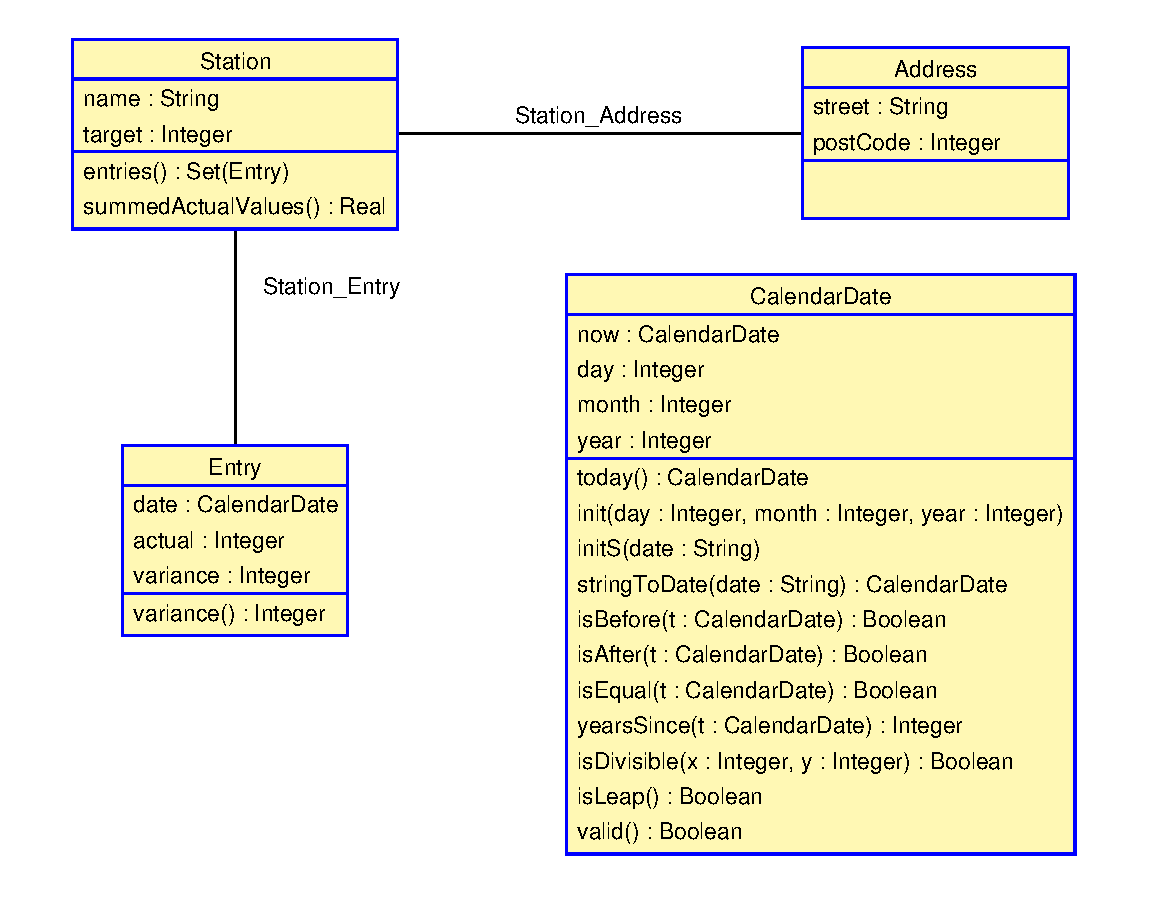
\includegraphics[scale=.4]{pics/USE_class_diagramm.pdf}
	\caption{Klassendiagramm für das Beispiel}
	\label{fig:Grafik2}
\end{figure}


\section{\uppercase{JUSE4Android}}
Dieser Abschnitt befasst sich mit der Anwendung JUSE4Android und untersucht die erstellte Anwendung sowie dessen Quellcode. 

%\begin{enumerate}[I]
%\item Wird das MVVM-Pattern berücksichtig?
%\item Kann einfache Berechnungslogik eventuell durch OCL-Constraints eingefügt werden?
%\item Ist der generierte Code kommentiert und wurden gängige Code-Konventionen eingehalten?
%\item Ist die Generierung nachvollziehbar und würde ein Entwickler ebenfalls so entwickeln?
%\item Wie anspruchsvoll gestaltet sich das anpassen oder das Ersetzen der Oberfläche 
%\item Gehen bei einer erneuten Generierung, manuelle Veränderungen am Code verloren?
%\begin{enumerate}[a]
%\item exestiert eine Möglichkeit für Geschützte Bereiche?\\
%\item Kann manueller Code von generiertem Code getrennt werden?
%\end{enumerate}
%\item Können unterschiedliche Berechnungslogiken definiert werden? Z.b. mittels \textit{Strategy} Entwurfsmuster 
%\end{enumerate}


\subsection{Vorstellung}
Das Tool JUSE4Android ist im Rahmen der Master-Arbeit \textit{Model-Driven Generative Programming for BIS Mobile Applications} von Luís Miguel Pires Teixeira da Silva entstanden und ermöglicht die Erstellung eine mobilen Business Information System (BIS) Anwendung für das Betriebssystem Android aus einer USE-Datei. Zum Persistieren von Daten wird das Objekt-Orientierte Datenbank-Framework \textit{db40} verwendet. Dieses wird nur bis zur Java-Version 1.6 unterstützt und stellt dementsprechend spezielle Anforderungen an das \textit{Android Software Development Kit}. Konkret bedeutet das, dass generierte BIS-Apps nur bis zum Android API-Level 17 lauffähig sind und mit der Betriebssystemversion Android 4.2 (\textit{Jelly Bean}) betrieben werden müssen. Da somit eine Menge moderner mobilen Geräte mit den generierten BIS-Apps nicht betrieben werden kann, ist dies als erheblicher Nachteil einzuschätzen.

\subsection{Untersuchung der erstellten Applikation}
\label{untApp}
Die generierte Anwendung wird durch die folgenden Schichten definiert: \textbf{Persistenz-Schicht, Präsentations-Schicht, Model-Schicht (Business Logik)}. Wie eine tiefere Analyse des Codes zeigte, wurden die Funktionen der Schichten nicht durchgängig eingehalten, was zu Brüchen der Schichtenarchitektur führt. So sind die eigentlichen Datenhaltungsobjekte (POJOs\footnote{POJO = Plain Old Java Object}) selbst für das Speichern und Löschen ihrer Daten aus der Datenbank verantwortlich und greifen dafür auf entsprechende Zugriffsobjekte zu. Bei einem lesenden Zugriff wird gänzlich auf die De­le­gie­rung an Zugriffsobjekte verzichtet und die Datenbank direkt angesprochen. Das Einbringen einer zusätzlichen Datenzugriffsschicht sowie die Verwendung des Fabrikmethoden-Entwurfsmuster zur Erstellung der POJOs würde die Lesbarkeit deutlich erhöhen. \textbf{Ein entwickler hätte es anders gemacht???}
Laut des Entwicklers wird konsequent das Model-View-View-Model Entwurfsmuster verwendet. Jedoch ist dies bei genauerer Betrachtung nicht nachvollziehbar. Zwar wird die Business-Logik von der View getrennt, jedoch werden die \textit{Activity Klassen\footnote{Klassen, die vom Typ Activity erben; übernehmen die Interaktionslogik für die Oberfläche und sind vergleichbar mit den sog. CodeBehind Klassen der xaml-Oberflächendefinitionen in Microsofts WPF-Framework }} als ViewModel verwendet. Diese beherbergen allerdings die Interaktionslogik für die korrespondierenden XML-Oberflächen Definitionen, genannt Layouts. Somit sind die vom Entwickler gewählten ViewModels Teil der Präsentations-Schicht, was im engeren Sinne der MVVM Definition widerspricht.
Dennoch wird eine lose Kopplung zwischen der eigentlichen Oberfläche und dem Model geschaffen. Diese eröffnet die Möglichkeit, Teile der Oberfläche zu ändern oder auszutauschen.\\
Das vorherrschende Architekturmuster ist das Naked-Object-Pattern. Dieses definiert 3 Prinzipien: 1.) Die gesamte Geschäftslogik wird in Domänen-Objekten gekapselt, 2.) Die Benutzeroberfläche ist eine direkte Repräsentation dieser Objekte und 3.) die Benutzeroberfläche kann oder wird direkt aus der Definition dieser Objekte erstellt. Diese 3 Prinzipien werden durch JUSE4Android vollständig umgesetzt. Zudem werden die Domänen-Objekte direkt in eine Objekt-Orientierte Datenbank gespeichert. Die Abbildung \ref{fig:Grafik3} verdeutlicht die Grundarchitektur des Naked-Objects-Patterns.\\
Der Programmfluss wird über die 4 grundlegenden Datenbankoperationen \textbf{C}reate \textbf{R}ead \textbf{U}pdate \textbf{D}elete gesteuert. Dabei werden neue Objekte sowohl in der Datenbank als auch der View verändert oder neu erstellt.\\ 
Die generierten Oberflächen verwenden das \textit{Master/Detail Flow} Layout, welches in der Lage ist, eine Liste von Items auf dem sogenannten \textit{Master} anzuzeigen. Bei der Auswahl eines Items erfolgt ein Übergang in die sogenannten \textit{Detail} Ansicht, in welcher Daten zu dem dazugehörigen Item präsentiert werden. Dieses Layout ermöglicht eine Anpassung der Oberfläche an verschiedene  Display-Größen.\\
In der generierten Anwendung sind die Oberflächen eine Eins-zu-eins Repräsentation der Business-Objekte. Dies entspricht den Forderungen des Naked-Object-Patterns.

\begin{figure}[!h]
	\centering
	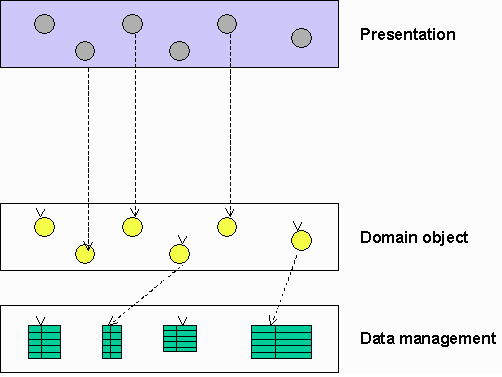
\includegraphics[scale=.5]{pics/NakedObjectPattern.png}
	\caption[Naked-Object-Pattern Architektur nach Richard Pawson, University of Dublin, Trinity College]{ Richard Pawson  \emph{\glqq Naked objects\grqq{}}; University of Dublin, Trinity College; 2004; Seite 24)}
	\label{fig:Grafik3}
\end{figure}

\subsubsection{Abbildung von Assoziationen und OCL-Constraints}
Eine Stärke modellgetriebener Entwicklungsprozesse liegt gemäß \cite{SWOT} in der Möglichkeit, Constraints formal mit Hilfe etablierter Standards auszudrücken. Bei generativen Ansätzen stellt sich die Frage, ob und in welchem Umfang ein Tool die Überprüfung der in einem abstrakten Modell beschriebenen Integritätsbedingungen umsetzt. Im Folgenden wird dieser Aspekt für die in der USE-Syntax spezifizierten Beziehungen und Constraints betrachtet. \\
Die Grundlage für etwaige Konsistenzprüfungen bilden POJOs, welche für jede definierte Klasse generiert werden.  
Für jede Assoziation, an der die entsprechende Klasse beteiligt ist, wird ein boolescher Zustand angelegt. Dieser drückt aus, ob ein Objekt die durch die Assoziation beschriebenen Kardinalitäten erfüllt. Für die Klasse Station ergeben sich beispielsweise die Zustände \textit{validPlace} (aus der Relation \textit{Station\_Address}) und \textit{validRecords} (aus der Relation \textit{Station\_Entry}). Ferner wird ein Zustand \textit{AssociationRestrictionsValid} zur Kennzeichnung der globalen Validität einer Objektes gespeichert. Diese ist gegeben, wenn alle Relationen modellkonform erfüllt werden. Bei der Ausführung von Create und Update-Operationen wird eine Verifikation durchgeführt; jedoch führt ein inkonsistenter Zustand nicht zum Abbruch der Operation. Objekte, welche nicht dem spezifizierten Schema entsprechen, werden von der Präsentations-Schicht als nicht valide gekennzeichnet.\\
Die im Abschnitt \ref{ssec:ocl} beschriebenen OCL-Bedingungen werden von JUSE4Android nicht auf algorithmischer Ebene abgebildet und folglich nicht überprüft.\cite[S.59]{SilvaMasterThesis} Dieser Umstand wird dadurch begründet, dass aktuelle Forschungsfragen auf diesem Gebiet noch nicht beantwortet sind. Beispielsweise ist unklar, welche Schicht die Umsetzung dieser Regeln übernehmen sollte oder ob ein Verifikation client- oder serverseitig erfolgen sollte. \cite[S.107]{SilvaMasterThesis} 
Die spezifizierten OCL-Ausdrücke finden sich auf Codeebene lediglich in Form von Kommentaren (oft mit dem Präfix \textit{TODO}) wieder. Beispielsweise erscheint Berechnungslogik als Java-Kommentar im Rumpf der entsprechenden Methode, während definierte Invarianten am Ende der Klasse eingefügt werden. Die in der USE-Syntax spezifizierten Ableitungen für Attribute können vom Tool nicht verarbeitet werden und wurden somit vor der Generierung aus dem PIM-Modell entfernt. 

%Im Falle der 1..* Assoziation zwischen den Klassen Station und Entry fungiert letztere als sogenannte \textit{Holder-Klasse}, da diese nur eine Instanz der Klasse Station beinhalten muss. \cite[S.86]{SilvaMasterThesis} Jedes POJO definiert die Methoden \textit{checkModelRestrictions()} und \textit{checkRestrictions()}, wobei erstere die Validität jeder einzelnen Relation und  Teilkomponenten  in welcher die jeweilig einzuhaltenden Kardinalitäten überprüft 

\subsubsection{Generierter Code und zusätzliche Funktionalität}
Der aus der USE-Definition generierte Code bedarf in den meisten Fällen einer manuellen Nachbearbeitung, um syntaktische Fehler der Generierung zu beheben. Diese äußern sich u.a. durch den Aufruf nicht deklarierter Variablen oder durch eine fehlerhafte Kommasetzung in Parameterlisten. 
Ebenfalls zeigten sich Probleme bei der Konfiguration des Build Paths in Form von nicht hinzugefügten Libraries.\\
Die Anwendung ist in eine aussagekräftige Paketstruktur gegliedert, wie Abbildung \ref{fig:Grafik4} zeigt. Außerdem hält sie die gängigen Code-Konventionen, wie beispielsweise die \textit{camelcase} Schreibweise ein. Dabei bilden die Getter-Methoden eine Ausnahme: diese besitzen nicht das Get-Präfix. Negativ muss ebenfalls erwähnt werden, dass der Code nur geringfügig kommentiert wurde und teilweise verschiedene Sprachen für die Kommentare verwendet wurden. Grundsätzlich erscheint der Code für einen fortgeschrittenen Java/Android Entwickler nachvollziehbar und verständlich. \\
Nur nach der Generierung sind manuelle Anpassungen oder das Hinzufügen komplexerer Funktionalität möglich. Diese werden dementsprechend bei einer erneuten Generierung wieder überschrieben. Ebenfalls ist keine Möglichkeit vorgesehen, geschützte Bereiche zu definieren. Auch das Auslagern von manuellem Code in separate Dateien kann nicht vorgenommen werden, da der gesamte Code - mit Ausnahme von wenigen vordefinierten Standardklassen - dynamisch durch die Applikation generiert wird. Somit ist eine Trennung von generiertem Code und manuellem Code nicht möglich. 


\begin{figure}[!h]
	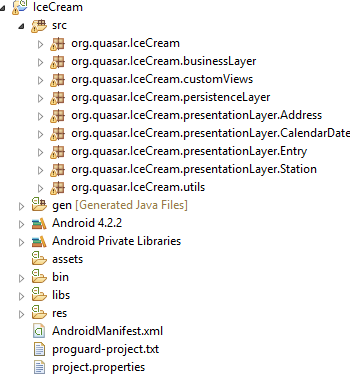
\includegraphics[scale=.6]{pics/Paket.png}
	\caption{Paketstruktur einer mittels JUSE4Android generierten Applikation}
	\label{fig:Grafik4}
\end{figure}



\subsubsection{Veränderungen der Benutzeroberfläche}
Wie bereits in Abschnitt \ref{untApp} beschrieben ist das verwendete Entwurfsmuster MVVM nicht vollständig erfüllt. Dennoch wurde festgestellt, dass es eine lose Kopplung zwischen der Business-Schicht und der Präsentations-Schicht gibt. Damit ist der Austausch vereinzelter Oberflächenkomponenten gewährleistet. Die Anpassung des Designs ist schon durch die Gestaltungsmechanismen des Betriebssystems Android ohne Probleme möglich. Ebenfalls können verwendete Grafiken einfach ausgetauscht werden. Theoretisch wäre der Austausch der gesamten Oberfläche auch möglich, jedoch entsteht dort ein Mehraufwand durch die nicht konsequente Verwendung des MVVM Architekturmusters. Bei der Auswechselung der Oberfläche müssten zum einen die in XML definierten Layout-Dateien verändert oder ausgetauscht werden, zum anderen müssten auch die \textit{Activity-Klassen} angepasst werden. Durch die Verwendung des Master/Detail Flow Layouts gehören zu jeder Oberflächenrepräsentation eines Objektes drei Klassen, welche die Anzeige steuern. Somit ist es nicht auszuschließen, dass es zu Inkonsistenzen im Programmfluss kommen könnte. Das Adaptieren einer neuen Oberflächengestaltung für eine durch JUSE4Android generierte Applikation ist demzufolge mit einem erheblichen Aufwand verbunden.\\
Im Rahmen dieser Arbeit wurde exemplarisch gezeigt, wie die Anpassung der Oberfläche möglich ist. Dabei wurde die Präsentation für die Darstellung der Varianz-Attributes leicht verändert. Wenn diese außerhalb des tolerablen Bereichs liegt, wird das anzeigende Feld rot eingefärbt, innerhalb des tolerablen Bereiches erscheint es grün. Um dies umzusetzen bedarf es eines manuellen Eingriffes in die \textit{EntryDetailFragment-Klasse}. Es wurde lediglich die Varianz mit dem Grenzwert verglichen und dann die Änderung der Textfarbe der Anzeigekomponente vorgenommen. Die Anpassung des ViewModel-Codes für die Umsetzung dieses Beispiels zeigt ebenfalls, dass hier das MVVM-Muster verletzt wurde.

JUSE4Android bietet Annotationen an, welche im USE-File verankert sind und durch welche geringfügig auf die View Einfluss genommen werden kann. SIEHE MASTERARBEIT Seite


\section{Zusammenfassung und Fazit}
JUSE4Anroid zu starr; möglicherweise geht es in die Richtung der Generierung von Softwarekomponenten, im Gegensatz zur Generierung einer vollständigen Applikation
individuelle Verständnisse der Entwickler, z.B. verschiedene Auffassungen darüber, wie Architekturmuster umgesetzt werden, könnten dazu führen, dass der Code schwierig nachvollziehbar wird
 Da somit eine Menge moderne Mobilen Geräte mit den generierten BIS-Apps kompatibel sind, ist dies als erheblicher Nachteil ein zu schätzen.
\vfill
\bibliographystyle{apalike}
{\small
\bibliography{bib/literature}}
\newpage
\section*{\uppercase{Anhang}}
\onecolumn
\begin{lstlisting}[caption={Vollständige USE-Spezifikation des IceCream Modells},label=lst:completeUSE]
------------------------------------------------------------------------
------------------------------------------------------------------------
model IceCream

-- description: Modified and extended version of the example for monitoring our ice-cream health,
-- 		see "GUI Architectures", by Martin Fowler (http://martinfowler.com/eaaDev/uiArchs.html)
-- author: Franziska Krebs, Tobias Franz, Jano Espenhahn; FH Brandenburg
-- last update: 31 January 2016
------------------------------------------------------------------------
------------------------------------------------------------------------

------------------------------------------------------------------------
-- CLASSES
------------------------------------------------------------------------

@StartingPoint(NameToDisplay="Station", ImageToDisplay="")
@list(name="1")
@creation(name="1", target="2")
@display(name="1",meanActualValue="2", meanVarianceValue="3",numberOfEntries="4",target="5")
@unique(name="1")
@domain()
class Station

	attributes

		name		: String
		target		: Integer
		numberOfEntries : Integer derive:entries()->size()
		meanActualValue : Real derive:calculateMeanActualValue()
		meanVarianceValue :Real derive:calculateMeanVarianceValue()
		
	operations
	
		entries(): Set(Entry) = self.records->asSet
	  
		calculateMeanActualValue() : Real = entries()->iterate(iterator : Entry; result : Real = 0 | result + iterator.actual)/(self.numberOfEntries) 
		pre:self.numberOfEntries>0

		calculateMeanVarianceValue() : Real = entries()->iterate(iterator :Entry; result : Real = 0 | result + iterator.variance)/(self.numberOfEntries) 
		pre:self.numberOfEntries>0
		
	constraints
	
		@TargetValueCannotBeNegative(rationale="The defined target value of a station cannot be smaller than 0")
		inv TargetValueCannotBeNegative:
			self.target>=0
		
		
		
end --Station

---------------------------------------------------------------------------------------

@StartingPoint(NameToDisplay="Address", ImageToDisplay="")
@list(street="1", postCode="2")
@creation(street="1", postCode="2")
@display(street="1", postCode="2")
@unique(street="1", postCode="2")
@domain()
class Address

	attributes

		street		: String
		postCode	: Integer
  
end --Address

---------------------------------------------------------------------------------------

@StartingPoint(NameToDisplay="Entry", ImageToDisplay="")
@list(date="1")
@creation(date="1",actual="2")
@display(date="1",actual="2",variance="3")
@unique(date="1")
@domain()
class Entry

	attributes

		date		: CalendarDate
		actual		: Integer
		variance	: Integer derive:calculateVariance()
	  
	operations

		calculateVariance(): Integer = self.actual - self.station.target
		pre:self.station <> null 
		
	constraints
	
		@ActualValueCannotBeNegative(rationale="The actual value measured at a station cannot be smaller than 0")
		inv ActualValueCannotBeNegative:
			self.actual>=0		
	
		@SelectedDateCannotBeInTheFuture(rationale="The selected date cannot be in the future.")
		inv SelectedDateCannotBeInTheFuture:
			self.date.isBefore(date.today()) or self.date.isEqual(date.today())
end --Entry

--------------------------------------------------------------
-- Library types
-- The below described class was taken from "Model-Driven Generative Programming for BIS Mobile Applications", da Silva, L. (2014)
--------------------------------------------------------------

@list()
@creation(year="1",month="2",day="3")
@display(year="1",month="2",day="3")
@unique(year="1",month="2",day="3")
@domain()
class CalendarDate

	attributes

		now: CalendarDate
		day: Integer
		month: Integer
		year: Integer

	operations

		today():CalendarDate = now

		init(day: Integer, month: Integer, year: Integer)
			begin
				self.day:= day;
				self.month:= month;
				self.year:= year
			end
			
		-- date format: yyyy-mm-dd
		initS(date: String)
			begin
				self.year:= date.substring(1,4).toInteger();
				self.month:= date.substring(6,7).toInteger();
				self.day:= date.substring(9,10).toInteger()
			end

		stringToDate(date: String): CalendarDate
			begin
			  declare 
					date_year : String,
					date_month : String,
					date_day : String;
					
				date_year:= date.substring(1,4);
				date_month:= date.substring(6,7);
				date_day:= date.substring(9,10);
				result:= CalendarDate.allInstances-> select(cd |
					cd.year=date_year.toInteger() and
					cd.month=date_month.toInteger() and 
					cd.day=date_day.toInteger())->asSequence()->first();
				if result.isUndefined() then
					result:= new CalendarDate('D'+date_year+date_month+date_day);
				  result.initS(date)
				end
			end
			
		isBefore(t: CalendarDate):Boolean = 
			if self.year = t.year then
				if self.month = t.month then
				self.day < t.day
				 else
				self.month < t.month
				 endif
			else 
				self.year < t.year
			endif

		isAfter(t: CalendarDate):Boolean =
			if self.year = t.year then
				if self.month = t.month then
					self.day > t.day
				 else
					self.month > t.month
				endif
			else 
				self.year > t.year
			endif

		isEqual(t: CalendarDate):Boolean =
			self.year  = t.year and
			self.month = t.month and
			self.day   = t.day

		yearsSince(t: CalendarDate):Integer =
			if self.month < t.month or
			   self.month = t.month and self.day < t.day then
					self.year - t.year -1
			else
				self.year - t.year
			endif

		isDivisible(x: Integer, y: Integer): Boolean = x div y * y = x
		
		isLeap(): Boolean =
			if isDivisible(self.year, 400) or isDivisible(self.year, 4) then
				true
			else
				if isDivisible(self.year, 100) then
					 false
				else
					if isDivisible(self.year, 4) then
						true
					else
						false
					endif
				endif
			endif
			
		valid(): Boolean =
				self.month>=1 and self.month<=12 and self.day>=1 and
				if self.isLeap() then
					self.day<=Sequence{31,29,31,30,31,30,31,31,30,31,30,31}->at(self.month)
				else 
					self.day<=Sequence{31,28,31,30,31,30,31,31,30,31,30,31}->at(self.month)
				endif

	constraints
	
		@DateIsValid(rationale="The current date must be a valid one")
		inv DateIsValid: self.valid()
		
		@CalendarDateObjectsContainDistinctDates(rationale="CalendarDate objects contain distinct dates")
		inv CalendarDateObjectsContainDistinctDates:
			CalendarDate.allInstances->
				isUnique(year.toString().concat('/').concat(month.toString()).concat('/').concat(day.toString()))
		
end --CalendarDate

------------------------------------------------------------------------
-- ASSOCIATIONS
------------------------------------------------------------------------
	
association Station_Entry between
	Station[ 1 ] role station
	Entry[ * ] role records
end

association Station_Address between
	Station[ 1 ] 
	Address[ 0..1 ] role place
end


\end{lstlisting}

Diese weicht ab von der tatsächlich zur Generierung verwendeten USE-Spezifikation 
 Annotationen sind JUSE4Android spezifisch und nicht Bestandteil der OCL


\twocolumn

\vfill
\end{document}

